\chapter{Software architecture}
Much of our work is focussed on porting software libraries such as the Tribler core, the anontunnels and libtorrent to Android. We are not developing a software product which is traditionally done for the bachelor end project. Instead we have developed an Android application called AT3 that we use to test the ported libraries. Additionally this software allows us to perform experiments such as bandwidth or CPU measurements.
In this chapter the software architecture of the AT3 application will be described. We will provide an overview of the different components and how they interact.

\section{Overview}
The general overview of the application is given in figure \ref{fig:overview}. The AT3 application is a very simple application used to test Tribler and the anontunnels on Android.

The main functionality is contained within the Tribler package, where we have created an extra \texttt{androidinterface.py} script. This script serves as an interface between the AT3 application and Tribler. It is used by the application's android service to start the anontunnels, download torrents using Tribler and obtain status information. 

\begin{figure}[h]
	\centering
	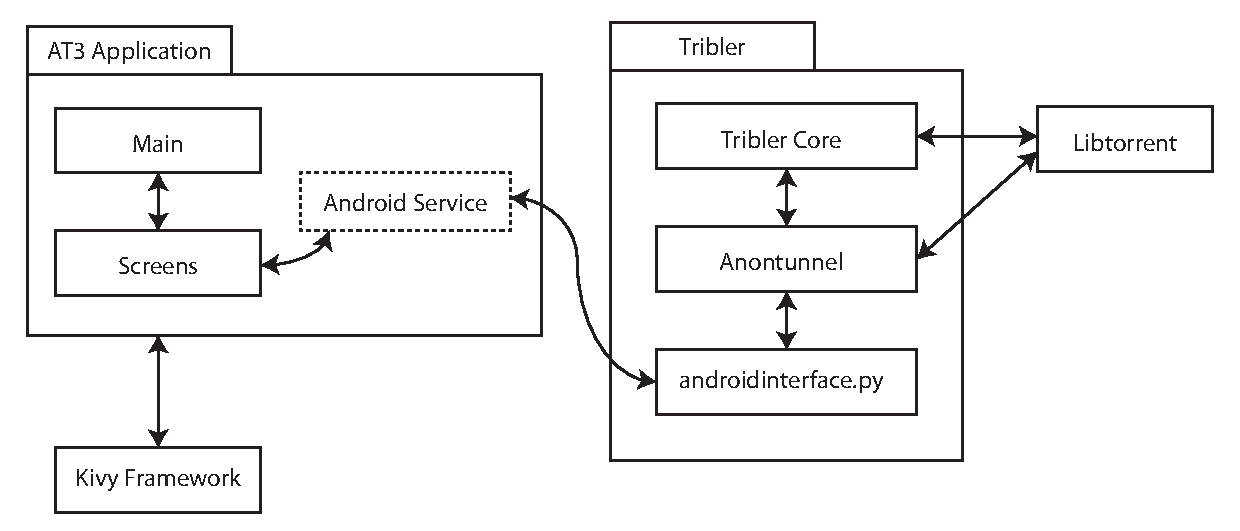
\includegraphics[width=\textwidth]{graphics/overview.pdf}
	\caption{A high level overview of the application}
	\label{fig:overview}
\end{figure}

\subsection{Kivy and Python for Android}
Kivy is a cross-platform application development framework written in Python. Kivy includes Python for Android, a build tool that can generate standalone Android applications that run Python code. We chose to use Kivy for the development of the application because all existing Tribler and anontunnel code is written in Python. Therefore this framework offers the most seamless integration with existing code. Kivy handles everything related to the user-interface. It hides away all the complexity of handling user input and displaying output.

\subsection{Tribler}
Tribler handles everything related to managing torrent downloads. The anontunnels, which are a part of Tribler, handle the anonymous tunnels over which we will download. These two components form the core part of our application.

Tribler is dependent on several python modules. You can find a package dependency graph for Tribler in appendix \ref{chp:dependency-tree}. One of the most important dependencies here is libtorrent, which is the library that handles torrent downloads.

\section{AT3 Application}
The AT3 application's main functionality is running the anontunnels and starting a test download. To do this, the application contains a start button which starts the anonymous tunnels and triggers a test download of 50 Megabyte. The sequence of this process is displayed in figure \ref{fig:sequencestart}.

\begin{figure}[h]
	\centering
	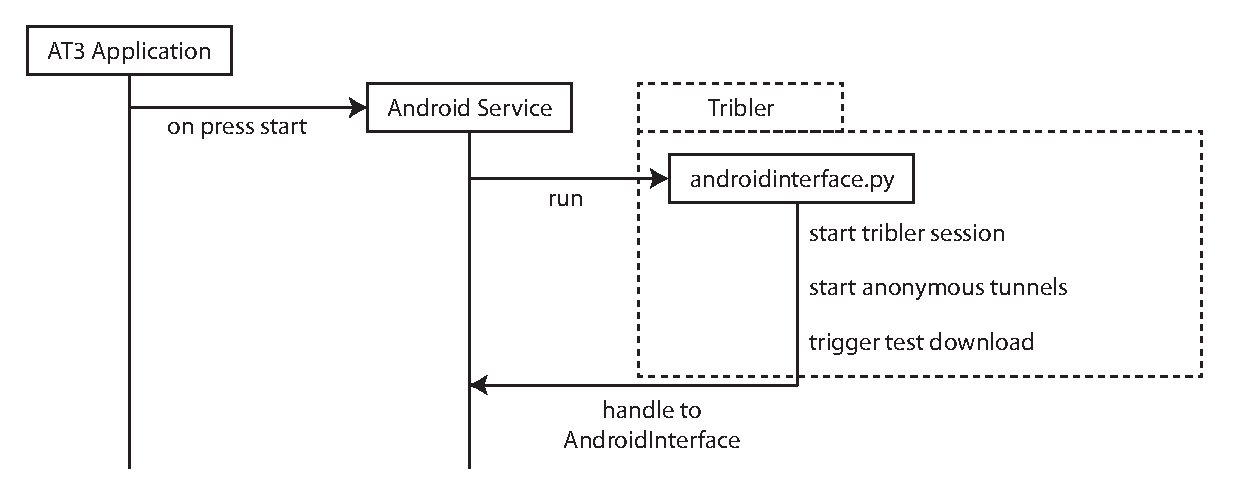
\includegraphics[width=\textwidth]{graphics/sequence-start.pdf}
	\caption{The sequence diagram of starting the anontunnels and triggering a 50 Megabyte torrent download}
	\label{fig:sequencestart}
\end{figure}

Periodically the application will want to obtain information about the status of the test download. Using a timer the application will request this information every second from the Android interface. Because the AT3 application and the android service run as different processes, the communication between them is facilitated by the Kivy OSC library. The sequence diagram of this process is displayed in figure \ref{fig:sequenceinfo}.

\begin{figure}[t!]
	\centering
	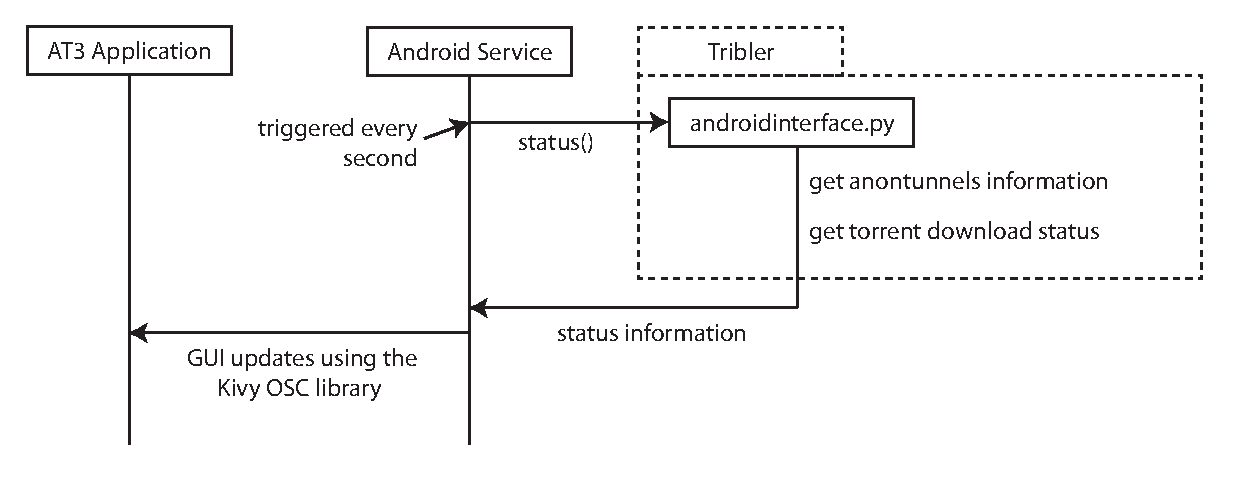
\includegraphics[width=\textwidth]{graphics/sequence-info.pdf}
	\caption{The sequence diagram of obtaining status information from the anontunnels and the test download}
	\label{fig:sequenceinfo}
\end{figure}

%\subsection{Code independence}
%We aim to not modify any code from the Python for Android framework or any other package we use in the application. When changes have to be applied, we try to minimize the amount of changes we have to do make.
%The reason we do this, is to ensure that future updates require no or minimal effort to be applied to the application.
%Besides that, we wish to create a pull request on Github with our work, so that the open source community can benefit from our work.
%Also, since our code will be independent from the Python for Android framework that we use, it will remain a "clean" environment so that anyone can reproduce the application with ease by simply downloading the framework and run our code from a separate place.

%\subsection{Code quality}
%It is our goal that at the end of each SCRUM sprint (see also section \ref{chp-Scrum}), we have a stable, improved product available. To ensure this, we make certain that the code on our master branch on Github always contains code that can produce a working application. Besides that, we also want to have at least one .apk application file of our stable version that can be installed on Android devices. For pull request, one other team members has to approve the pull request before it is merged into the master.
%More on how we ensure code quality can be found in section \ref{codeQuality}.

%\section{Software architecture}
 %The software architecture of our application is designed in such a way that it should be capable of running on most Android devices. Any Android device running on the ARM architecture and having the Android SDK API level 14 or higher installed should be able to run this application.
 
%\subsection{Programming languages and programs}
%\label{programminglang}
%This application is written in Python, Kivy script and shell script, making use of text editor programs such as gedit and Sublime. With gedit, one can easily adapt scripts as it's the default text editor on the Ubuntu operating system. Sublime is used for editing and creating Python code, because this program contains auto indentation and colors to separate e.g. functions from variables. This speeds up the development and with the colors one can easily separate different things to minimize errors.
%As Python for Android uses the Kivy framework to make the Graphical User Interface (GUI), we also use Kivy to create our GUI's with.
%Finally, shell scripts are used to create so called recipes and building scripts that run certain commands. More about these recipes can be found in \ref{iteration1}.

%\subsection{Tests}
%As we are largely dependent on third party code, we will first make sure that the core functionality of these third party codes also functions on PC's. The Tribler team has set up a download test than can be run in order to check if everything works as it should. This test is run on the Tribler PC version, which also contain these third party libraries.

%We assume that third party libraries are tested by their respective authors, and that these tests are covering and passing before any of these libraries are released.
%Our shell scripts will be tested as well. Our scripts are divided into dependency files (configuration files) and functionality files with methods. Methods that check for critical components return exit statuses which can be tested.

%\subsection{Maintaining code quality}
%\label{codeQuality}
%To uphold the code quality we make use of pull requests to merge git branches into the master branch, which contains the stable and final version of each sprint. When someone would like its code to be merged with the code on the master branch, he has to create a pull request that must be reviewed by another team member. During this review, this team member will closely watch for missing comments, wrong style, unclear or too complicated code and the completeness of tests when tests are required.

%The style of the code for Python should be conform to PEP 8. For shell scripts we follow the rules of indenting and commenting as described by various parties such as Google and Linux kernel.
%All scripts must contain good and relevant comments following the guidelines if they exist, variable names should be clear and meaningful of their purpose and of course the code style must match the guidelines as well.

%When a pull request is approved and can be automatically merged, it is merged into the master branch. When the master is updated, a new and stable version is created. All other branches that are being worked on should pull the master branch into theirs to ensure that their code is not behind and can be automatically merged without merge conflicts when they are ready to create a pull request.

%\subsection{Package architecture}
%As mentioned in section \ref{programminglang} we make use of recipes. Each recipe downloads and installs a package that is required for the application to work. Most of the time, a package depends on other packages or is used by another package as dependency. As more packages are added to the application, the dependencies become more complicated.
%To maintain and overview the structure and dependencies of the packages, we've created a package dependency graph. See appendix \ref{chp:dependency-tree}.